% By J. Leon, Beerware licence
\documentclass[tikz,border=10pt]{standalone}
\usepackage{tikz}
\usetikzlibrary{positioning, fit, arrows.meta, shapes}

% To avoid repeating same command several times
% Command \empt{var1}{var2}
\newcommand{\empt}[2]{$#1^{\langle #2 \rangle}$}

\begin{document}

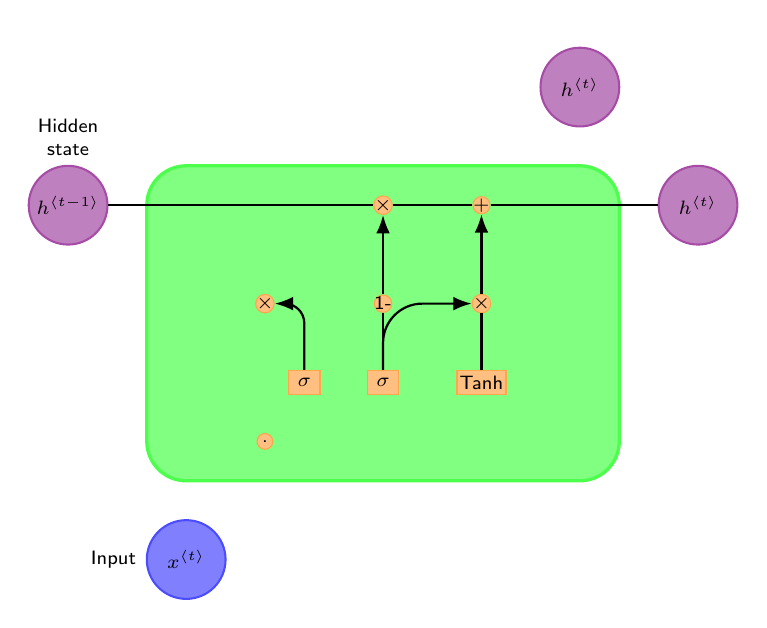
\begin{tikzpicture}[
    % GLOBAL CFG
    font=\sf \scriptsize,
    >=LaTeX,
    % Styles
    cell/.style={% For main box
        rectangle,
        rounded corners=5mm,
        draw=green!70,
        very thick,
        fill = green!50,
    },
    operator/.style={% For operators (such as + and x)
        circle,
        draw=orange!70,
        inner sep=-0.5pt,
        minimum height =.2cm,
        fill=orange!50,
    },
    function/.style={% For functions
        ellipse,
        draw=orange!70,
        inner sep=1pt,
        fill=orange!50,
    },
    cellstate/.style={% For external inputs and outputs
        circle,
        draw=red!70,
        line width = .75pt,
        minimum width=1cm,
        inner sep=1pt,
        fill=red!50,
    },
    input/.style={% For external inputs and outputs
        circle,
        draw=blue!70,
        line width = .75pt,
        minimum width=1cm,
        inner sep=1pt,
        fill=blue!50,
    },
    hidden/.style={% For external inputs and outputs
        circle,
        draw=violet!70,
        line width = .75pt,
        minimum width=1cm,
        inner sep=1pt,
        fill=violet!50,
    },
    gt/.style={% For internal inputs
        rectangle,
        draw=orange!70,
        minimum width=4mm,
        minimum height=3mm,
        inner sep=1pt,
        fill=orange!50,
    },
    mylabel/.style={
        font=\scriptsize\sffamily
    },
    ArrowC1/.style={% Arrows with rounded corners
        rounded corners=.25cm,
        thick,
    },
    ArrowC2/.style={% Arrows with big rounded corners
        rounded corners=.5cm,
        thick,
    },
    every text node part/.style={
        align=center
    },
    ]

    % Draw
    % Draw cell
    \node [cell, minimum height =4cm, minimum width=6cm] at (0,0){} ;

    % Draw inputs named ibox#
    \node [gt] (ibox1) at (-1.0,-0.75) {$\sigma$};
    \node [gt] (ibox2) at (0,-0.75) {$\sigma$};
    \node [gt] (ibox3) at (1.25,-0.75) {Tanh};

    % Draw operators named mux#, add# and func#
    \node [operator] (mux1) at (0,1.5) {$\times$};
    \node [operator] (add1) at (1.25,1.5) {+};
    \node [operator] (mux2) at (-1.5,0.25) {$\times$};
    \node [operator] (minusone) at (0,0.25) {1-};
    \node [operator] (mux3) at (1.25,0.25) {$\times$};
    \node [operator] (point) at (-1.5,-1.5) {.};

    % Draw external inputs named as basis c, h, x
    \node[hidden, label={[mylabel]Hidden\\ state}] (h) at (-4,1.5) {\empt{h}{t-1}};
    \node[input, label={[mylabel]left:Input}] (x) at (-2.5,-3) {\empt{x}{t}};

    % Draw external outputs named as basis c2, h2, x2
    \node[hidden, label={}] (h2) at (2.5,3) {\empt{h}{t}};
    \node[hidden, label={}] (h3) at (4,1.5) {\empt{h}{t}};
    %\node[hidden, label={}] (h2) at (4,-1.5) {\empt{h}{t}};

    % Connect all
    % Intersections and displacements are used
    \draw [ArrowC1] (h) -- (mux1) -- (add1) -- (h3);
    %Drawing arrows

    %Inputs
    %\draw [ArrowC1] (h -| ibox1)++(-0.5,0) -| (ibox3);
    %\draw [ArrowC1] (h -| ibox2)++(-0.5,0) -| (ibox2);
    %\draw [ArrowC1] (h -| ibox3)++(-0.5,0) -| (ibox3);

    % Internal
    \draw [->, ArrowC1] (ibox1) |- (mux2);
    \draw [->, ArrowC2] (ibox2) -- (minusone) -- (mux1);
    \draw [->, ArrowC2] (ibox2) |- (mux3);
    \draw [->,ArrowC2] (ibox3) -- (mux3) -- (add1);
    %\draw [->, ArrowC2] (ibox4) |- (mux3);
    %\draw [->, ArrowC2] (mux2) -- (add1);
    %\draw [->, ArrowC1] (add1 -| func1)++(-0.5,0) -| (func1);
    %\draw [->, ArrowC2] (func1) -- (mux3);

    % Outputs
    %\draw [-, ArrowC2] (mux3) |- (h2);
    %\draw (h3 -| x2) ++(0,-0.1) coordinate (i1);
    %\draw [-, ArrowC2] (h2 -| x2)++(-0.5,0) -| (i1);
    %\draw [-, ArrowC2] (i1)++(0,0.2) -- (x2);

\end{tikzpicture}

\end{document}
